\begin{frame}
    \frametitle{Performance?}
    \begin{columns}
        \begin{column}[t]{0.48\textwidth}
            \begin{itemize}
                \setlength\itemsep{.8em}
                \item We compared results in H2S molecule
                \item Normalizing Flows greatly improved stretching case (Fig.~\ref{fig:enrs_stretch_2D})
                \item RNVP behaves similarly to IResNet
                \item Possibly perform better on higher dimensional data
            \end{itemize}
        \end{column}
        \begin{column}[t]{0.48\textwidth}
            \begin{figure}
                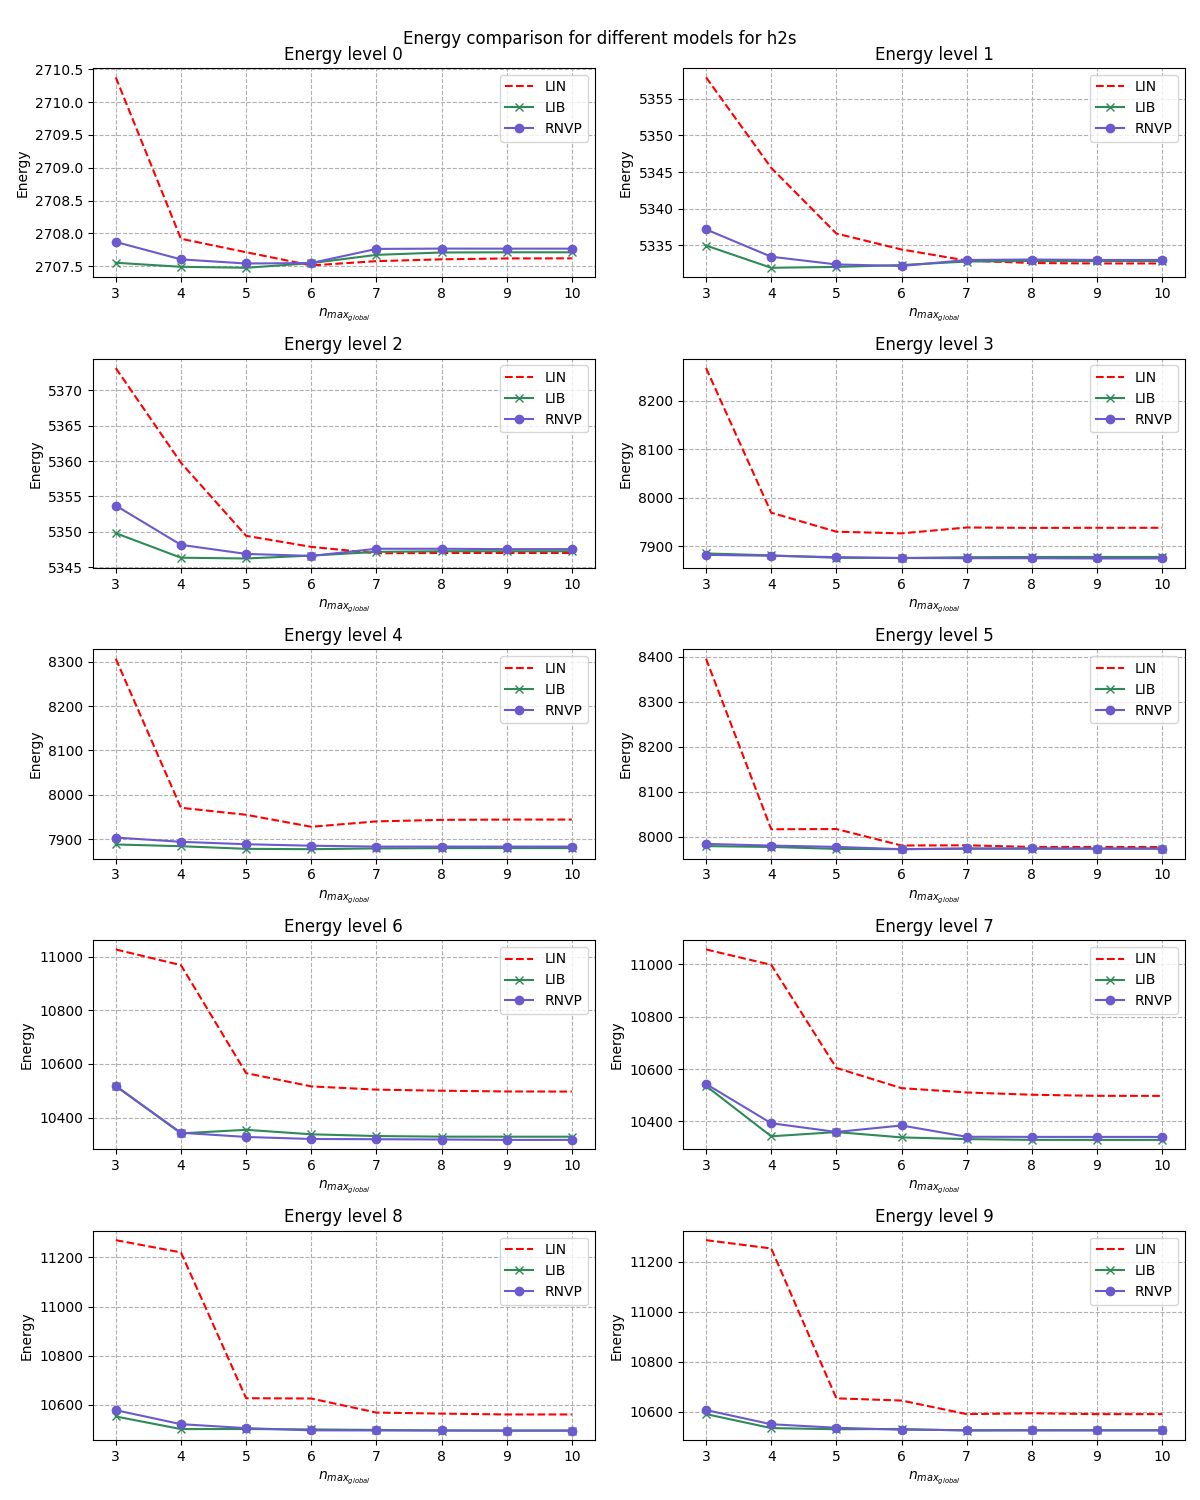
\includegraphics[width=\textheight]{img/enrs_stretch_2D.png}
                \caption{Stretching case for H2S molecule}
                \label{fig:enrs_stretch_2D}
            \end{figure}
        \end{column}
    \end{columns}
\end{frame}